\documentclass[10pt,a4paper]{article}
\usepackage[utf8]{inputenc}
\usepackage{amsmath}
\usepackage{amsfonts}
\usepackage{graphicx}
\usepackage{amssymb}
\usepackage[numbers,sort&compress]{natbib}
\usepackage[left=2cm,right=2cm,top=1.1cm,bottom=2cm]{geometry}
\usepackage[spanish]{babel}
\author{Orlando Lázaro Ruiloba Torres}
\title{Tarea 1 Optimización de Flujo en Redes}
\date{\today}

\usepackage{listings}
\usepackage{color}

\definecolor{dkgreen}{rgb}{0,0.6,0}
\definecolor{gray}{rgb}{0.5,0.5,0.5}
\definecolor{mauve}{rgb}{0.58,0,0.82}

\lstset{
	frame=tb,
	language=Python,
	aboveskip=3mm,
	belowskip=3mm,
	showstringspaces=false,
	columns=flexible,
	basicstyle={\small\ttfamily},
	numbers=none,
	numberstyle=\tiny\color{gray},
	keywordstyle=\color{blue},
	commentstyle=\color{dkgreen},
	stringstyle=\color{mauve},
	breaklines=true,
	breakatwhitespace=true,
	tabsize=3
}

\begin{document}
\maketitle

\section{Grafo simple no dirigido acíclico}

Un ejemplo de la aplicación práctica de un grafo simple no dirigido acíclico, pudiera ser el organigrama de una empresa o institución, de acuerdo a \cite{art1}, ya que este constituye una representación gráfica de la estructura de la misma, donde los vértices o nodos son los puestos de trabajo, y los arcos representan las relaciones existentes entre ellos ya sea directa o indirectamente.\vspace{.4cm} 

El código en Python se muestra a continuación:

\lstinputlisting[language=Python]{grafo_simple_no_dirigido_aciclico.py}

\begin{center}

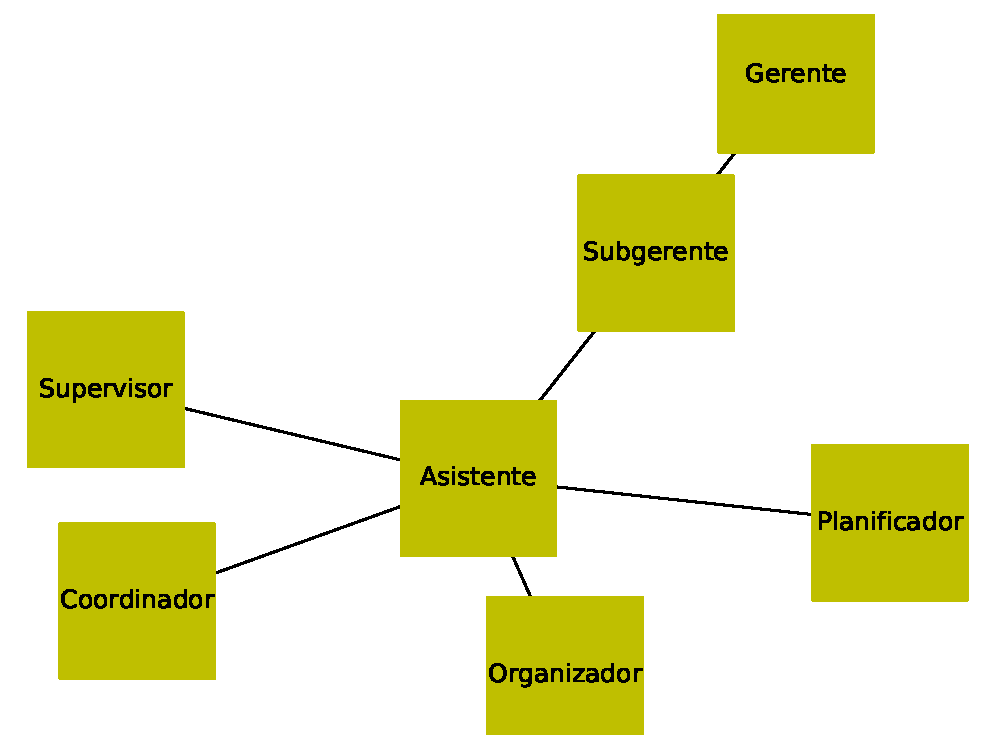
\includegraphics[scale=0.4]{GNDA}

\end{center}

\section{Grafo simple no dirigido cíclico}

Un ejemplo práctico de la aplicación de este tipo de grafo, pudiera ser la representación de una red de distribución directa según \cite{art2}, donde los productos salen de la fábrica y van directamente al consumidor final, los vértices serían los clientes y la fábrica, y los arcos el camino que los une, debiendo volver finalmente al vértice que representa el punto inicial (fábrica), repitiendo este proceso tantas veces como sea necesario, sin seguir un orden específico.\newpage

El código en Python se muestra a continuación:

\lstinputlisting[language=Python]{grafo_simple_no_dirigido_ciclico.py}

\begin{center}

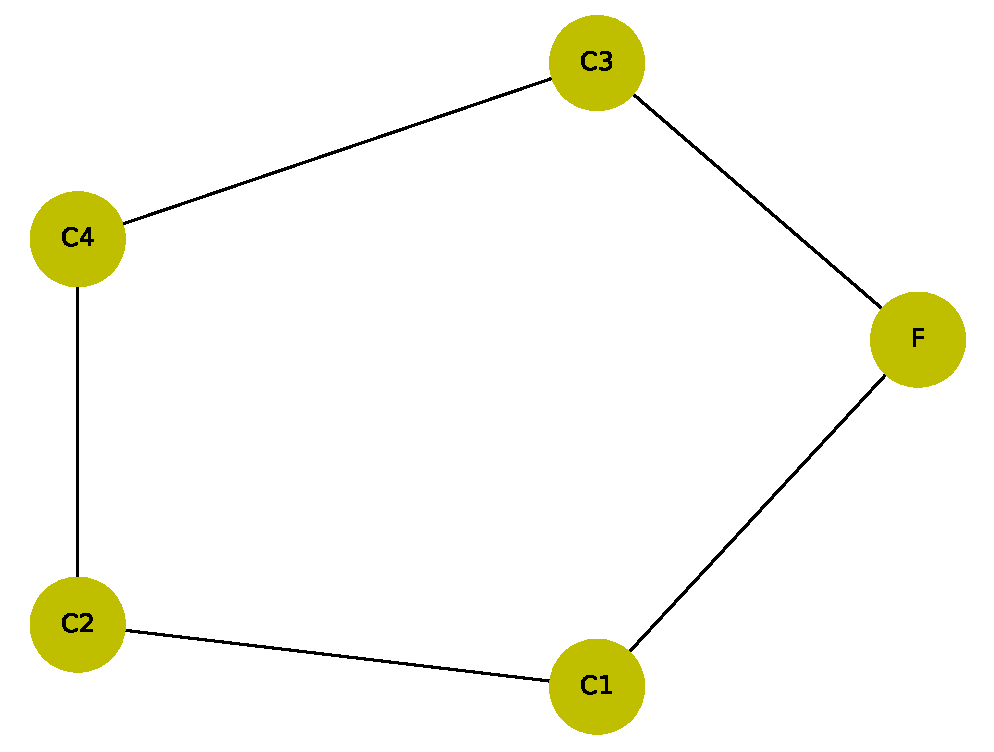
\includegraphics[scale=0.4]{GNDC}

\end{center}

\section{Grafo simple no dirigido reflexivo}

Para este caso, un ejemplo en la práctica sería, de acuerdo a \cite{art2} una red de carreteras que interconecta diferentes ciudades, donde los vértices serían las ciudades y los arcos las carreteras que las unen.\vspace{.4cm}

El código en Python es:
 
\lstinputlisting[language=Python]{grafo_simple_no_dirigido_reflexivo.py}

\begin{center}

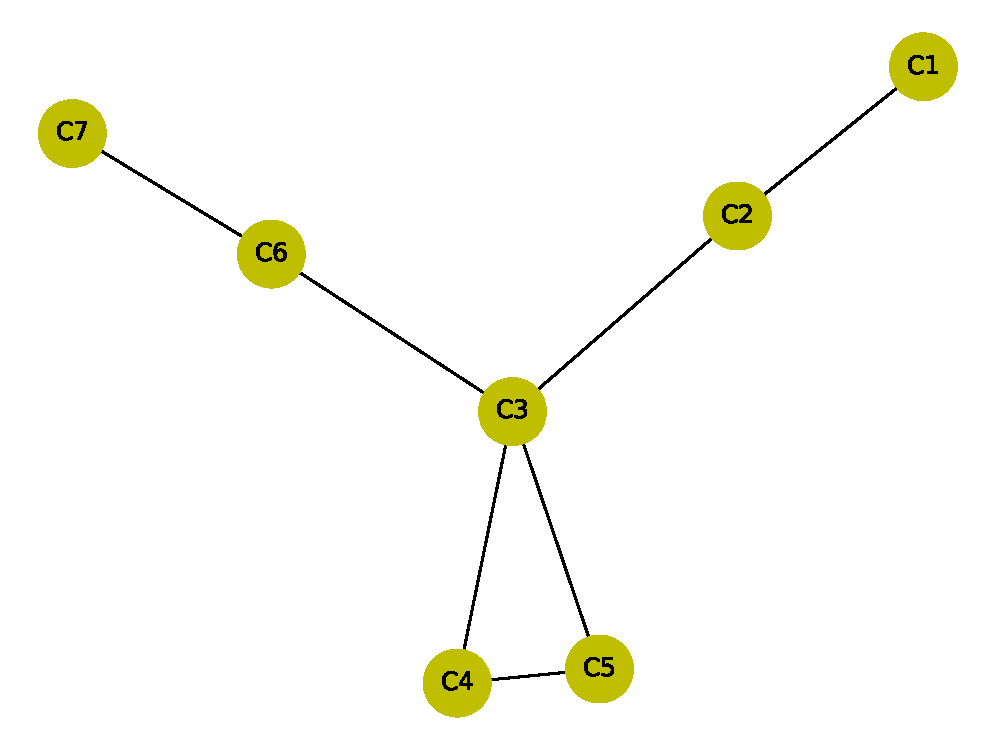
\includegraphics[scale=0.4]{GNDR}

\end{center}

\section{Grafo simple dirigido acíclico}

Un ejemplo para este caso en particular, pudiera ser de acuerdo a \cite{art2}, una estructura jerárquica de datos, donde los vértices corresponden a entidades y los arcos a las relaciones existentes entre las mismas.\vspace{.4cm}

El código en Python es el siguiente:

\lstinputlisting[language=Python]{grafo_simple_dirigido_aciclico.py}

\begin{center}

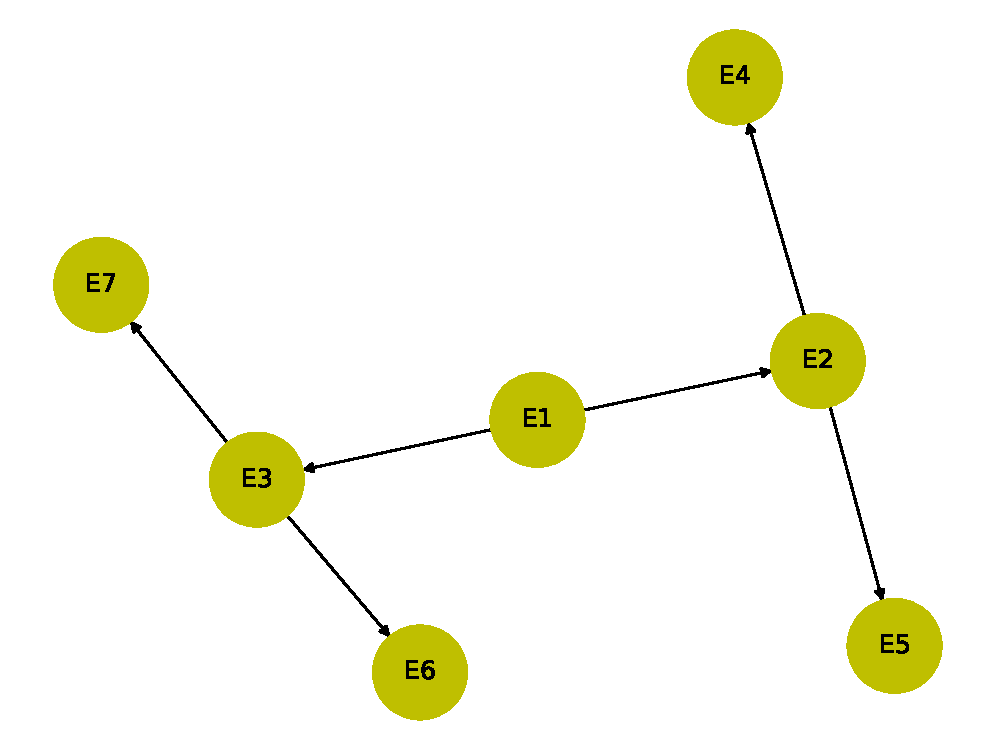
\includegraphics[scale=0.4]{GDA}

\end{center}

\section{Grafo simple dirigido cíclico}

Un ejemplo en la práctica de este tipo de grafo de acuerdo a \cite{art2}, puede ser la representación del proceso para la confección en masa de un determinado producto en una fábrica, ya que esto implica el desarrollo de varios subprocesos que tienen una secuencia determinada y que se van a repetir un número específico de veces, donde los vértices serían los subprocesos y los arcos la relación ordenada existente entre ellos.\vspace*{.4cm}

El código en Python se presenta a continuación:

\lstinputlisting[language=Python]{grafo_simple_dirigido_ciclico.py}

\begin{center}

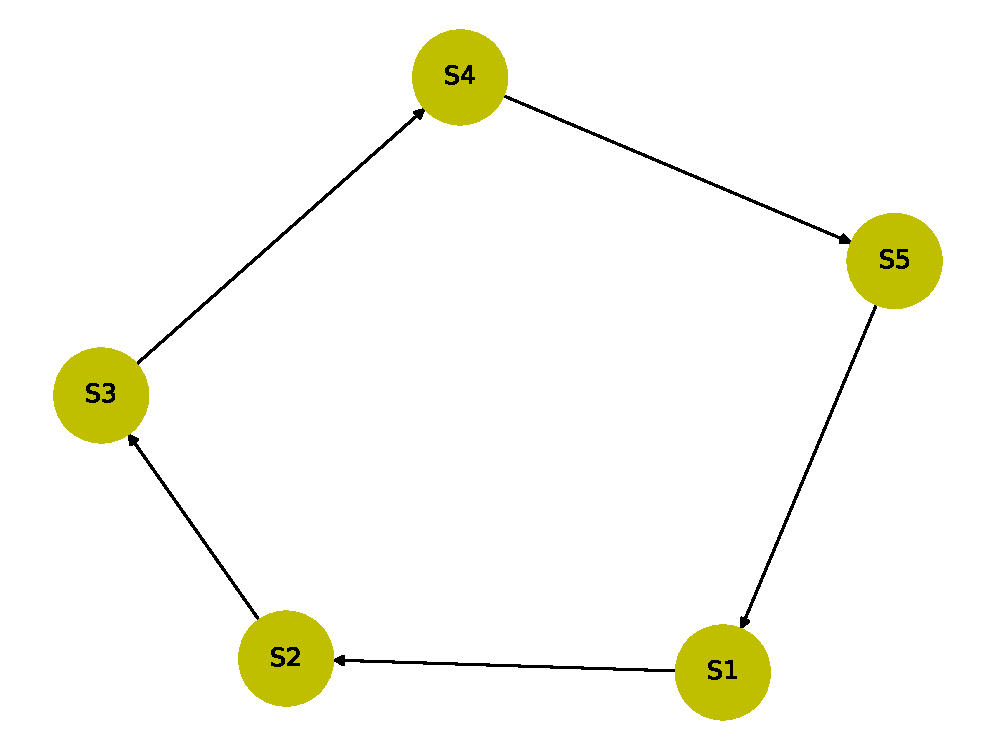
\includegraphics[scale=0.4]{GDC}

\end{center}

\section{Grafo simple dirigido reflexivo}

Un ejemplo en la práctica de este tipo de grafo se vería reflejado de acuerdo a \cite{art2}, en una red de aviación donde los vértices serían las ciudades o países a visitar y los arcos representan el camino recorrido por el avión.\vspace{.4cm}

El código en Python es:

\lstinputlisting[language=Python]{grafo_simple_dirigido_reflexivo.py}

\begin{center}

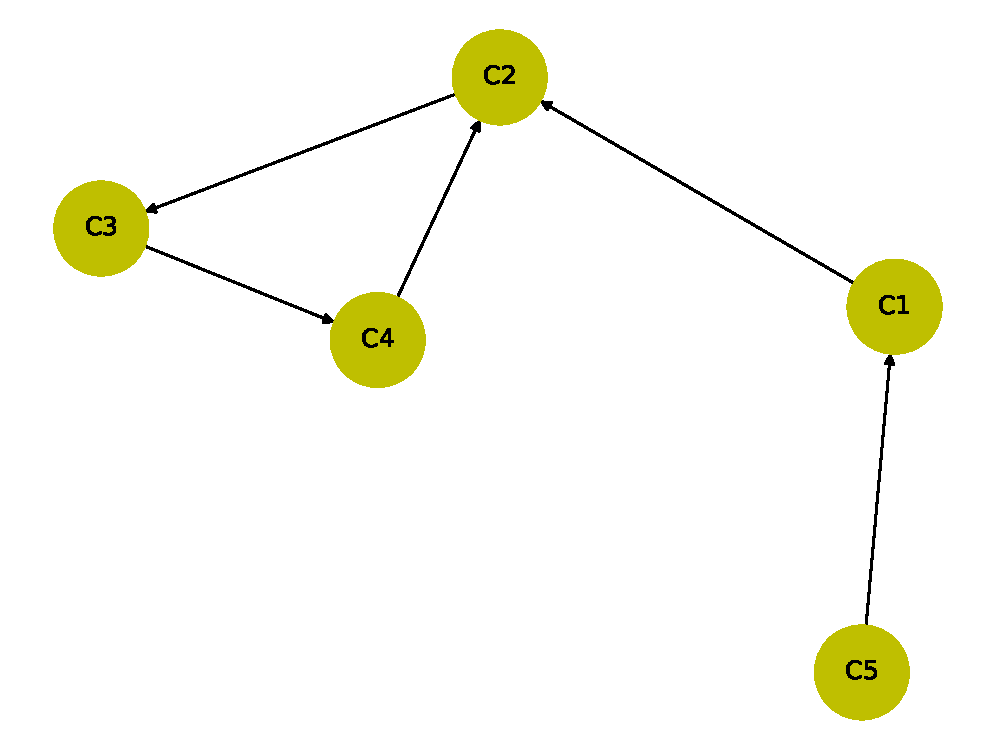
\includegraphics[scale=0.4]{GDR}

\end{center}


\section{Multigrafo no dirigido acíclico}

Un ejemplo en la práctica de este tipo de multigrafo según lo expuesto en \cite{art4} pudiera ser el caso de un museo, que desarrolla una exposición en varias salas al unísono, donde la situación ideal sería poder transitar por todas las salas sin tener que pasar necesariamente dos veces por la misma, se consideran las salas como los vértices, y las aristas, los caminos que las unen.\newpage

El código en Python es:

\lstinputlisting[language=Python]{multigrafo_no_dirigido_aciclico.py}

\begin{center}

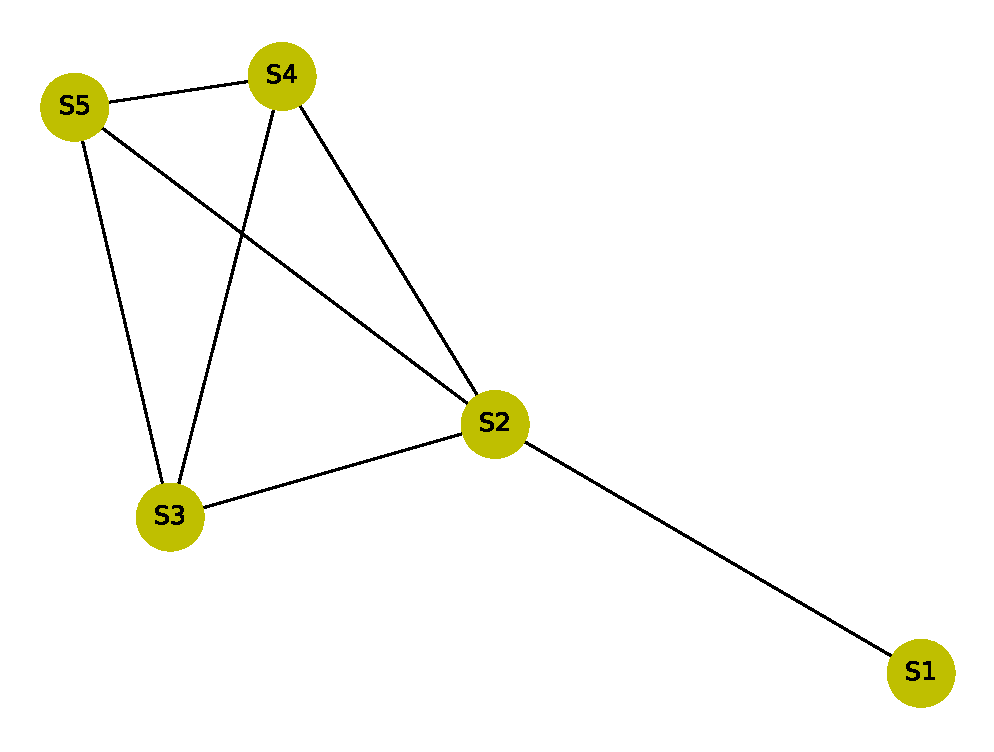
\includegraphics[scale=0.4]{MNDA}

\end{center}

\section{Multigrafo no dirigido cíclico}

Un ejemplo práctico para este caso en particular, se evidencia de acuerdo a \cite{art3} en la generación de redes tipo pequeño mundo, concepto que de hecho es muy común y nada alejado de nuestras experiencias diarias, ya que poco después de conocer a un extraño, uno se da cuenta de que tiene un amigo en común con él, este concepto se basa en el principio de los seis grados de separación, que establece que entre cualesquiera dos personas del mundo, existe una media de seis conexiones de amistad.\vspace{.4cm}

El código en Python es:

\lstinputlisting[language=Python]{multigrafo_no_dirigido_ciclico.py}

\begin{center}

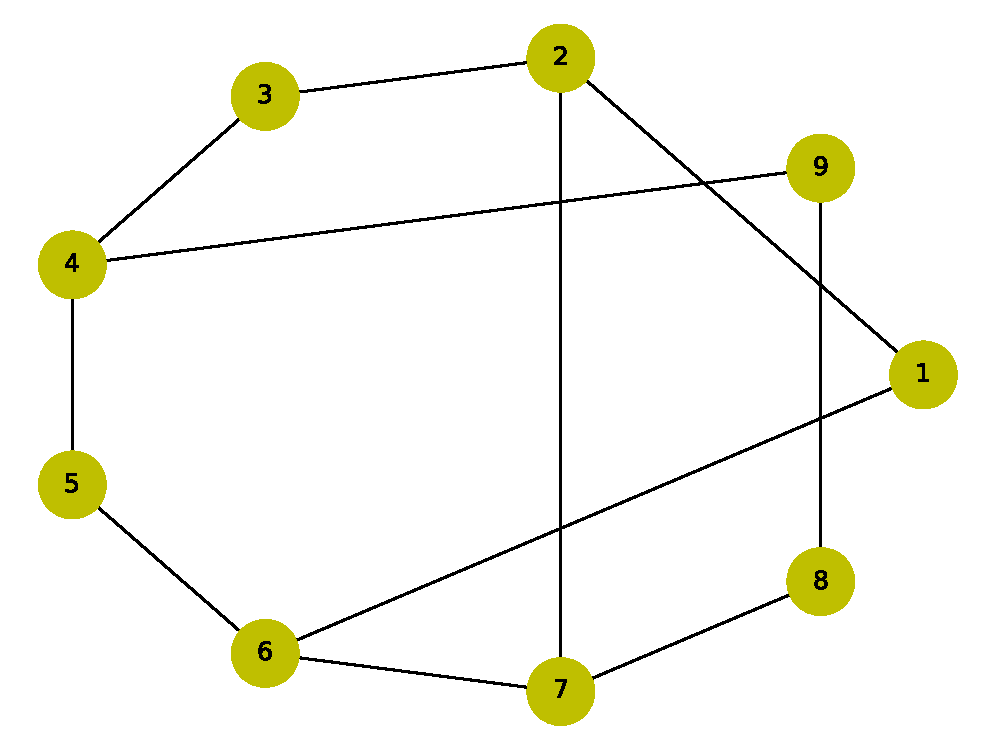
\includegraphics[scale=0.4]{MNDC}

\end{center}

\section{Multigrafo no dirigido reflexivo}

Un ejemplo de este tipo de multigrafo en la vida cotidiana puede ser según lo expuesto en \cite{art7} una red social de personas, donde los vértices pueden representar hombres o mujeres, personas con diferentes nacionalidades, edades, ingresos, etc y los arcos pueden simbolizar amistad, proximidad geográfica, conocimiento profesional, entre otros.\vspace{.4cm}

El código en Python es:

\lstinputlisting[language=Python]{multigrafo_no_dirigido_reflexivo.py}

\begin{center}

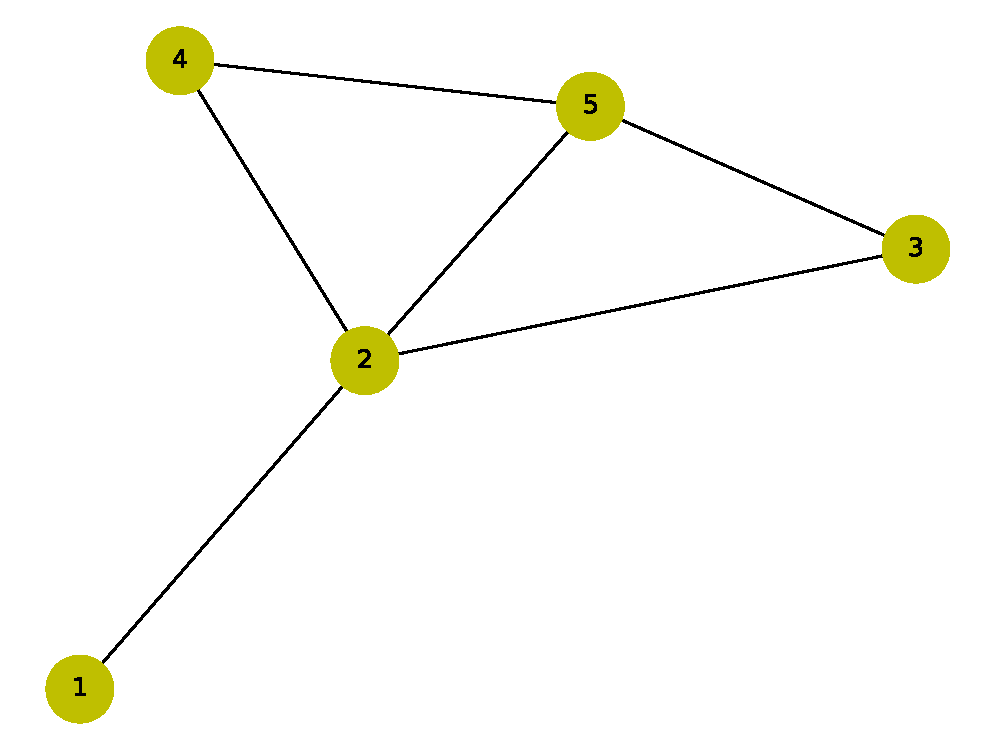
\includegraphics[scale=0.4]{MNDR}

\end{center}
 
\section{Multigrafo dirigido acíclico}

Un ejemplo de una aplicación práctica de este tipo de multigrafo se pone de manifiesto en una pequeña red de electricidad entre cinco ciudades, donde los vértices serían las ciudades y el tendido eléctrico serían las aristas que las unen, en el caso de C4, recibe la energía a través de C3 en dos canales que alimentan a la totalidad de la ciudad.\newpage

El código en Python es:

\lstinputlisting[language=Python]{multigrafo_dirigido_aciclico.py}

\begin{center}

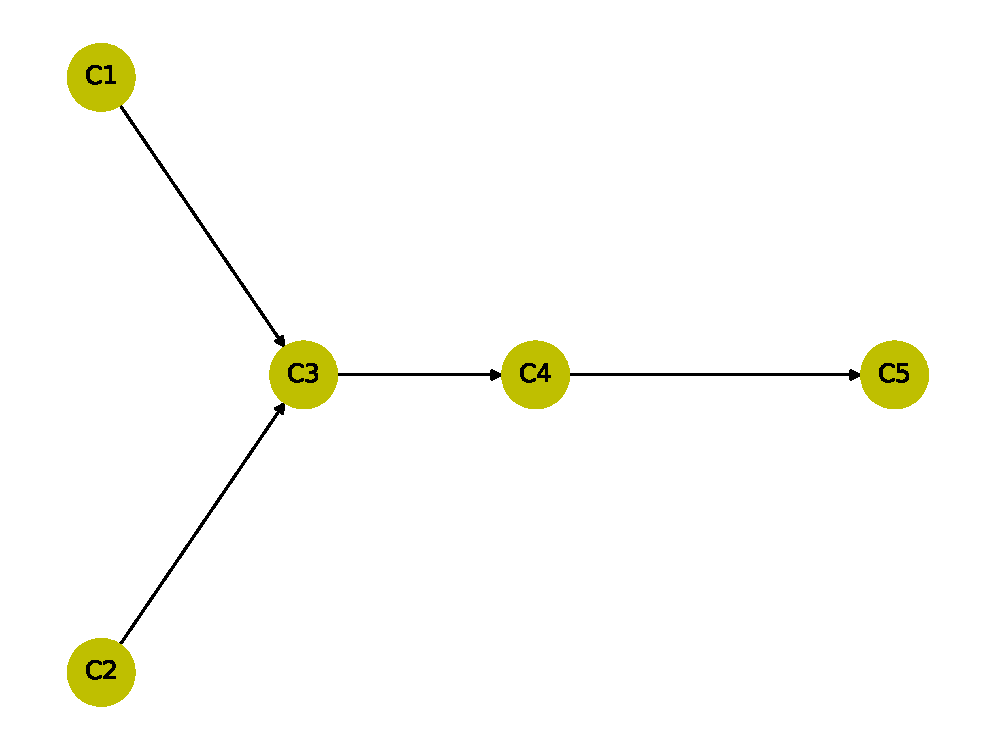
\includegraphics[scale=0.4]{MDA}

\end{center}

\section{Multigrafo dirigido cíclico}

Un ejemplo de la puesta en práctica de este tipo de multigrafo pudiera ser según \cite{art5} la modelación de 5 estaciones de una red de metro, donde cada estación da lugar a un vértice y los arcos simbolizan el camino de ida y vuelta entre cada una de las estaciones.\vspace{.4cm}

El código en Python es:

\lstinputlisting[language=Python]{multigrafo_dirigido_ciclico.py}

\begin{center}

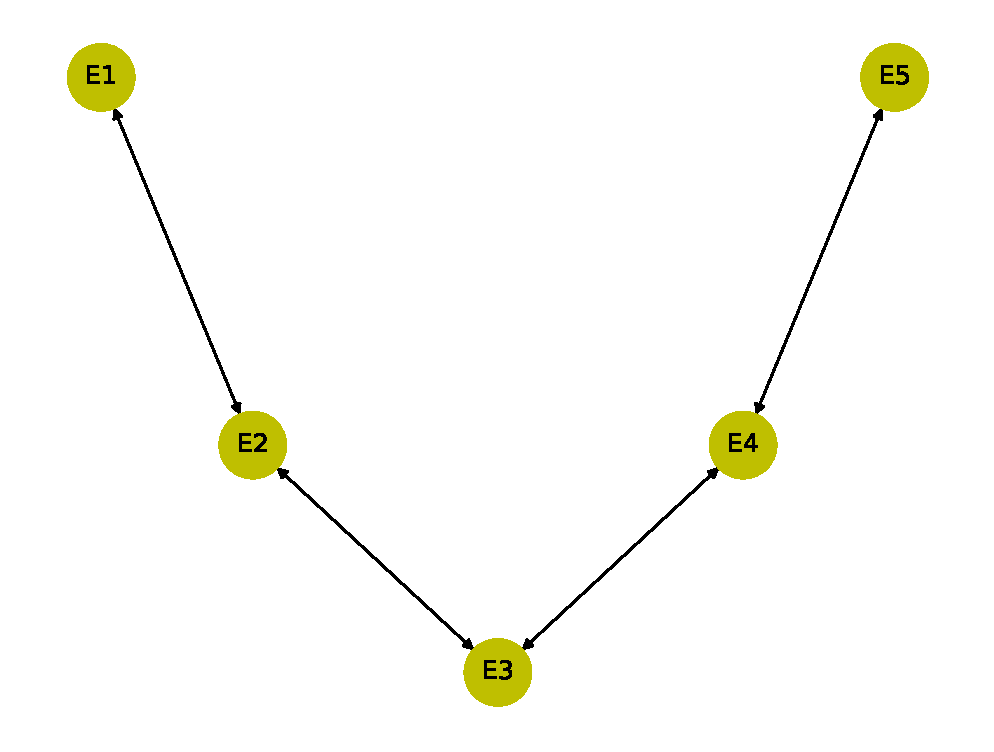
\includegraphics[scale=0.4]{MDC}

\end{center}

\section{Multigrafo dirigido reflexivo}

Un ejemplo de la puesta en práctica de este tipo de multigrafo pudiera ser según se muestra en \cite{art6} una red de comunicación en donde los vértices son los dispositivos de red y los arcos son los medios de networking (medios de transmisión basados en cobre o fibra óptica) que aseguran el envío y recepción de los mensajes y la información a través de la red de datos.\vspace{.3cm}

El código en Python es:

\lstinputlisting[language=Python]{multigrafo_dirigido_reflexivo.py}

\begin{center}

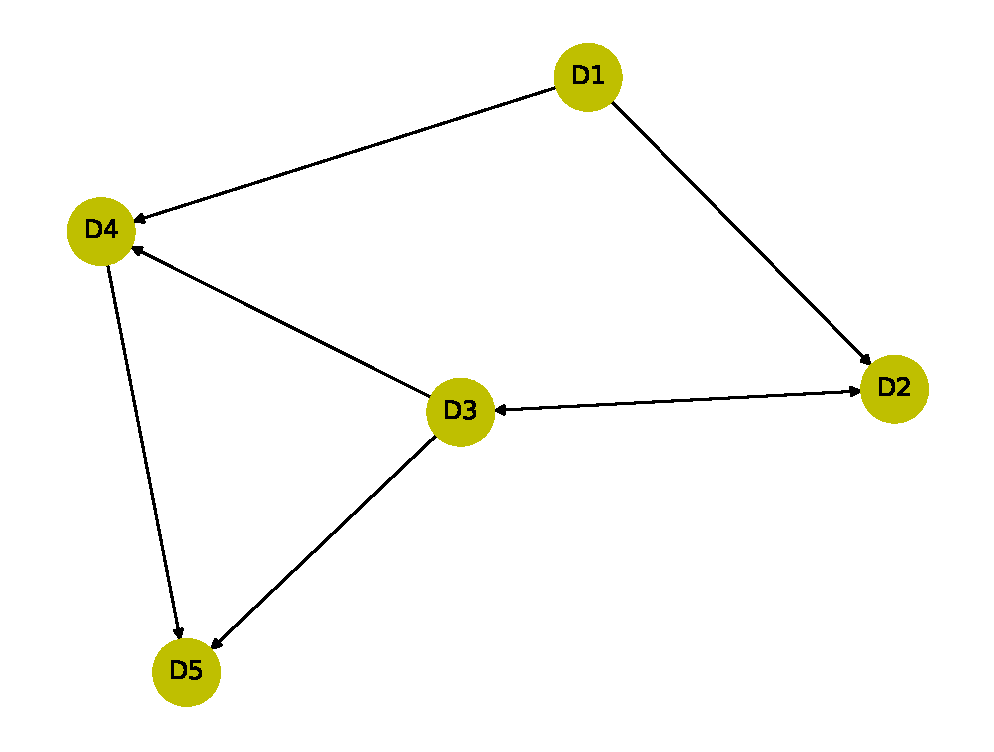
\includegraphics[scale=0.4]{MDR}

\end{center} 

\bibliography{Referencias}

\bibliographystyle{plainnat}

\end{document}